\section{Evaluation}

To evaluate the use of Chord to serve DNS data,
we used data from the study by Jung {\em et al.}\ on
a simulated network with 1000 DDNS nodes.
For the test, we turned off replication of records.
We did not simulate node failures,
so the only effect of replication would be to serve
as {\em a priori} caching.
Since the network is a fair amount smaller than the expected
size of a real Chord ring, replication would
bias the results in our favor because of the increased caching.

We first inserted answers to all the successful queries into the Chord network
and then ran a day's worth of successful queries
(approximately 260,000 queries),
measuring storage balance, load balance while answering
queries, and the number of RPCs required to perform each lookup.
The day's queries are heavy tailed.
There were about 120,000 distinct queries.  Of these, 93,100 appeared
just once.
Only 141 queries were executed more than a hundred times,
and only two were executed more than a thousand times.
The most common query, for {\em lcs.mit.edu}'s SOA record,
was executed 4219 times.

To simulate failed DNS queries, we started a similar network, did not insert
any data, and executed a day's worth of unresolved queries (approximately
220,000 queries), measuring
load balance and RPC counts.
These queries were distributed similarly to the successful queries.
Of 17,000 distinct queries, 8,000 were executed only once.
Only 165 queries were executed more than a hundred times,
and only eight were executed more than a thousand times.
The most common query, for {\em 39.246.224.209.in-addr.arpa}'s
PTR record, was executed 82,000 times.

Finally, to simulate popular entries, we ran what we called the ``slashdot test,''
inserting one record and then fetching it a hundred thousand times.

All three tests began each lookup at a random node in the Chord network.

\begin{figure}
\epsfig{file=figures/ok.store.eps}
\caption{
Storage balance for 120,000 records later used as answers to
260,000 queries.
The graph shows a cumulative distribution for the number 
of records stored on each node.
Perfect balance would place the same number of records
on each node, making the cumulative distribution a vertical line
around 120.}
\label{fig:store}
\end{figure}

For the successful queries test, we inserted approximately 120,000
records to serve as answers to the 260,000 queries.
Figure~\ref{fig:store} shows that the median number of
records stored per node is about 120, as expected.
The distribution is exponential in both directions because
Chord nodes are randomly placed on a circle and store data
in proportion to the distance to their next neighbor clockwise
around the circle.  Irregularities in the random placement cause
some nodes to store more data than others.
The two nodes that stored in excess of 800
records (824 and 827) were both responsible for approximately
0.8\% of the circle, as compared with an expected 
responsibility of 0.1\%.
Even so, this irregularity drops off exponentially in both
directions, and can be partially addressed by having servers
run multiple nodes in proportion to their storage capacities.
We conclude that DDNS does an adequate job of balancing
storage among the peers.

\begin{figure}
\epsfig{file=figures/both.fetch.eps}%,angle=270,width=3in}
\caption{Load balance for the three tests.
The graph shows a cumulative distribution for the number
of RPCs served by each node during the test.}
\label{fig:both-rpc}
\end{figure}

DHash's block caching helped provide load balance as
measured by RPCs served per node.
As shown in figure~\ref{fig:both-rpc},
in the successful query test, nodes served RPCs in
approximate proportion to the number of records they stored.
Specifically, each node serves each of its popular blocks about
ten ($\log_2 1000$) times; after that, the block is cached
at enough other nodes that queries will find a cached copy
instead of reaching the responsible server.
A similar argument shows that very quickly every node has
a copy of incredibly popular blocks, as evidenced by the
Slashdot test: after the first few thousand requests, virtually
every node in the system has the record cached, so that
subsequent requests never leave the originating node.

For the unsuccessful query test, nodes served RPCs in 
proportion to the number of queries that expected the
desired record to reside on that node.
This does a worse job of load balancing since there is
no caching; for example, the node responsible for the
PTR record for {\em 39.246.224.209.in-addr.arpa} was
heavily loaded due to the 82,000 queries for that record.

\begin{figure}
\epsfig{file=figures/hops.eps}%,angle=270,width=3in}
\caption{Client load to perform lookups. 
The graph shows a cumulative distribution for the number
of hops required for each lookup.}
\label{fig:hops}
\end{figure}

Figure~\ref{fig:hops} shows the number of RPCs required
by a client for various lookups.
Successful queries and unsuccessful queries have the same
approximately random distribution of hop counts, except
that successful queries usually end earlier due to finding
a cached copy of the block.
Since the slashdot record got cached everywhere very quickly,
virtually all lookups never left the requesting node.

\begin{figure}
\epsfig{file=figures/03.ok.lat.eps}
\caption{Lookup latency distribution for successful queries.}
\label{fig:oklat}
\end{figure}

Figure~\ref{fig:oklat} shows the distribution of latency
for successful lookups in the one-day DNS trace. A very small
fraction of lookups took more than 1000 ms to complete. 
This was mostly caused by requesting DNS data from name servers
that are behind slow links. If DNS were to be deployed over 
Chord, lookups that takes too long will be terminated and 
the request sent to the next replica for the data.

\begin{figure}
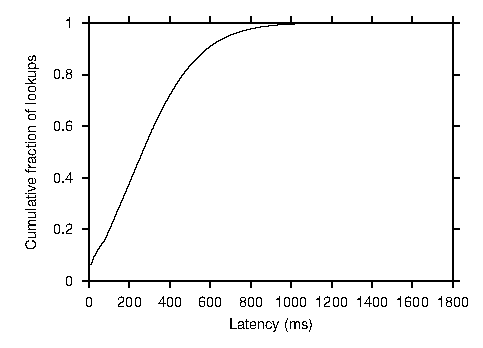
\epsfig{file=figures/imaglat.ok.eps}
\caption{Imaginary latency to perform lookups.}
\label{fig:imaglat}
\end{figure}

Imaginary latency in Figure~\ref{fig:imaglat}. 
XXX I'm not sure what you did here, Russ.

\begin{figure}
\epsfig{file=figures/hopslat.eps}
\caption{Estimated latency per lookup.}
\label{fig:hopslat}
\end{figure}

Since only a miniscule fraction of name servers are slow
(from Figure~\ref{fig:oklat}) we used the middle 95\% range
of latency as the sample size to estimate the lookup latency
over DDNS. For each lookup, we add up $x$ sampled latencies,
where $x$ is the number of hops in that lookup. We plot the 
estimated mean lookup latency and the error bars for one 
standard deviation in both directions over all lookups consisting
of $x$ hops. Figure~\ref{fig:hopslat} shows the estimated 
lookup latency for successful queries on DDNS. Since the mean
number of hops for a successful query is around 5 
(from Figure~\ref{fig:hops}), the estimated mean latency 
is approximately 350 ms. This is worse than the average mean in
current DNS (XX ms). However, the worst case in DDNS is only 800 ms,
compared to XX ms in the current DNS.

%RSC: what does this mean?
% Do a measure of how long it takes to converge to good load 
% balancing when there is a burst of lookups for 1 (or more)
% popular names. Compare that to the slashdot effects now.

%\subsubsection{Latency}

%We cannot perform a fair measurement of latency so we will do an
%analysis based on counting number of hops between servers
%and combining that with real latency to current root DNS servers.

%XXAdding keys to resource records make them bigger
%XXPublic key cryptography is an expensive operation. 
%DDNS computes pub keys every time.

%DDNS is not going to disappear without an answer for a lookup,
%unlike in the current DNS. So we can't really compare this, but should
%mention about it.
